% !TEX root = ../thesis-example.tex
%
\chapter{Background}\label{sec:diffusion}

This chapter introduces the necessary background that is relevant to our work. In the following, we provide an overview of generative modeling methods in machine learning. Then, we present diffusion models as the generative method we would like to improve. Finally, we present a few density ratio estimation techniques as this will be the backbone of our refinement techniques. 

\section{Generative modeling}\label{sec:related:sec1}


Generative modeling denotes a branch of unsupervised learning that aims to construct a \textbf{model} of the data $x \in \mathcal{X}$. By considering that a dataset can be described by a probability distribution $p(x)$ - that we call a \textit{target} distribution - the challenge is to estimate such a distribution by finding the best set of parameters able to approximate it, among a set of potential \textit{generators} $G$. A notable ability of generative models is generating new data instances that resemble the observed data, by sampling from the \textit{estimated} distribution $\hat{p}(x)$ .
Through the rapid development of deep learning and the abundance of training data over the past decade, generating data has attained impressive performances across various data types, often in high dimensions, such as language \citep{openai2024gpt4technicalreport}, visual data such as images \citep{rombach2022highresolutionimagesynthesislatent} and videos \citep{videoworldsimulators2024}, and speech \citep{wavenet}. This progress went on to include different types of input, termed as multimodal generative models \citep{Suzuki_2022}.

\subsection{Theoretical formulation}
\begin{assumption}\label{ass:1}
    We assume that the domain of interest $\mathcal{D} \subset \mathcal{X}$ is governed by a probability distribution  $P_{\mathcal{D}}$ of density $p(x)$.
\end{assumption}
Given a training dataset \textbf{x} of $n$ points sampled i.i.d from $P_{\mathcal{D}}$, we would like to approximate the target density $p(x)$ with a parametric family of models. Our focus is on deep learning based approaches involving neural networks. Thus, given a foxed architecture, we denote by $\Theta$ the set of all weights represented by this architecture.
The traditional approach in density estimation with a parametric family of models is maximum likelihood estimation (MLE) or maximum a posteriori (MAP). The likelihood function $L(\theta \mid X)$ of a parameter $\theta \in \Theta$ given the data $X$ is defined as the joint probability of the observed data:
\begin{equation}
L(\theta \mid X) = \prod_{i=1}^n p(x_i \mid \theta).
\end{equation}

The maximum likelihood estimation problem involves finding the parameter $\theta$ that maximizes the likelihood function. Formally, we define the MLE of $\theta$ as:
\begin{equation}
\hat{\theta}_{\text{MLE}} = \arg\max_{\theta} L(\theta \mid X).
\end{equation}

In practice, it is often more convenient to work with the log-likelihood function, since the logarithm is a monotonic function. The log-likelihood of $\theta$ is given by:
\begin{equation}
\ell(\theta \mid X) = \log L(\theta \mid X) = \sum_{i=1}^n \log p(x_i \mid \theta).
\end{equation}

Thus, the MLE problem can also be formulated as maximizing the log-likelihood:
\begin{equation}
\hat{\theta}_{\text{MLE}} = \arg\max_{\theta} \ell(\theta \mid X).
\end{equation}
This problem can be generalized as a \textbf{density estimation} problem, using the concept of statistical divergences.
\begin{definition}\label{def:divergence}
    Given two probability distributions $P,Q$ over $\mathcal{X}$, a statistical divergence $D(.\|.)$ is a function :
    \begin{equation}
D(P \| Q) : \mathcal{P} \times \mathcal{Q} \rightarrow [0, \infty),
\end{equation}
where $\mathcal{P}$ and $\mathcal{Q}$ are the spaces of probability distributions on $\mathcal{X}$.

The function $D(P \| Q)$ satisfies the following properties:
\begin{itemize}
  \item Non-negativity: $D(P \| Q) \geq 0$ for all $P, Q \in \mathcal{P} \times \mathcal{Q}$.
  \item Identity of indiscernibles: $D(P \| Q) = 0$ if and only if $P = Q$ almost everywhere.
\end{itemize}
\end{definition}
The absence of the symmetry assumption excludes statistical divergences from being metrics. However, they are still effective in comparing probability distributions. Table \ref{tab:divergences} provides examples of statistical divergences of interest in our work.
\begin{table}[ht]
\centering
\caption{Generic Mathematical Expressions for Statistical Divergences}
\[
\begin{array}{|>{\bfseries}m{4cm}|m{10cm}|}\label{tab:divergences}
\hline
\textbf{Category} & \textbf{Generic Mathematical Expression} \\
\hline
\textbf{F-Divergences} & $D_f(P \| Q) = \int q(x) f\left(\frac{p(x)}{q(x)}\right) \, dx$ \\
\hline
\textbf{Renyi Divergences} & $D_{\alpha}(P \| Q) = \frac{1}{\alpha - 1} \log \int p(x)^\alpha q(x)^{1-\alpha} \, dx$ \\
\hline
\textbf{Bregman Divergences} & $D_\phi(\mathbf{p}, \mathbf{q}) = \phi(\mathbf{p}) - \phi(\mathbf{q}) - \langle \nabla \phi(\mathbf{q}), \mathbf{p} - \mathbf{q} \rangle$ \\
\hline
\end{array}
\]
\end{table}
Given a divergence $D$, a target density $p(x)$ and a family of parametric models $\Theta$, one can formulate the optimal density as the solution of :
\begin{equation}\label{eq:density_est}
    \hat{\theta} = \arg\min_{\theta \in \Theta} D(\hat{p}(x; \theta) \| p(x))
\end{equation}
Once the density is estimated, one can sample from a generator $G_{\hat{\theta}}$ function, according to the type of generative model used.
\subsection{Sampling from an estimated distribution}
In this subsection, we give three examples of the training and sampling schemes of popular generative models in deep learning.
\begin{itemize}
    \item \textbf{Generative adversarial networks (GANs)} \citep{goodfellow2014generativeadversarialnetworks} consist in simultaneaous training of two different networks having opposing objectives. The first network, called a discriminator $D_{\phi}$ discriminates between samples from the \textit{target} distribution and samples from another distribution. The second network, called a generator $G_{\theta}$, attempts to sample from the target distribution to fool the discriminator. Essentially, this consists in solving the following min-max problem \citep{nowozin2016fgantraininggenerativeneural}, given a convex, lower-semi continuous function $f$:
    \begin{equation}\label{eq:f_gan}
        \min_{\theta} \max_{\phi} V(D_{\phi}, G_{\theta}) = \mathbb{E}_{x \sim p(x)}[D_{\phi}(x)] - \mathbb{E}_{z \sim p_{\theta}(z)}[f^*(D_{\phi}(G_{\theta}(z)))]
    \end{equation}
    where $f^*$ denotes the Fenchel conjugate of $f$. This objective function corresponds to a variational lower bound on the $f$-divergence between the target distribution and the generator distribution \citep{Nguyen_2010}. Once this objective is optimized, the generator $G_{\theta}$ is then used to sample from the estimated distribution. While GANs are celebrated for their sample quality, they often suffer from mode collapse which leads to a lack of diversity \citep{10.1145/3283254.3283282},and an unstable training due to the double optimization induced by the training objective.
    \item \textbf{Variational autoencoders (VAEs)} \citep{kingma2022autoencodingvariationalbayes} are probabilistic generative models that frame the problem of data generation as a Bayesian inference task. The key idea is to encode inputs into a latent (hidden) space via a neural network, and then decode from this latent space back to the data space. The encoder learns a distribution $q_{\phi}(z|x)$ over the latent space conditioned on the input data $x$, aiming to approximate the true but intractable posterior $p(z|x)$. The decoder, parameterized by $\theta$, attempts to reconstruct the input $x$ from the latent variable $z$, sampled from $q_{\phi}(z|x)$. The loss function of a VAE can be described as:
    \begin{align}
        \mathcal{L}(\theta, \phi; x) = -\mathbb{E}_{q_{\phi}(z|x)}[\log p_{\theta}(x|z)] + D_{\text{KL}}(q_{\phi}(z|x) \| p(z)),
    \end{align}
    where the first term is the expected log likelihood of the decoder (which measures reconstruction accuracy), and the second term is the Kullback-Leibler divergence between the encoded distribution and a prior distribution (typically a standard normal), acting as a regularizer. The VAE thus balances between accurate reconstruction and a meaningful, well-structured latent space. Sampling from a VAE involves passing randomly drawn samples from the prior $p(z)$ through the decoder to generate new data points that resemble the training data. As opposed to GANs, VAEs have a mass covering advantage but lack the quality provided by GAN generated samples. A recent line of work attempts to combine both strengths of these models to provide both quality and diversity to the generation process \citep{gimenez2022unifiedfdivergenceframeworkgeneralizing}.
    \item  \textbf{Diffusion Models} are another class of generative models that have recently gained significant attention due to their ability to generate high-quality samples. Similar to VAEs, diffusion models operate over a latent space and involve a gradual transformation process. However, instead of encoding and decoding directly, diffusion models start by gradually adding noise to the data until a simple noise distribution is reached, effectively 'diffusing' the data. By inspiring from theories in nonequilibrium thermodynamics, this process is then reversed to generate new samples from noise by learning to denoise through a series of steps. This is conceptually similar to the way VAEs attempt to map data to and from a latent space, but diffusion models do so over many more transformations, providing a smoother mapping and potentially richer generative capabilities. In the following section, we delve more in the theory behind diffusion models as it represents the main focus of our work.
\end{itemize}

\section{Diffusion models}\label{sec:related:sec2}
In this section, we derive the theoretical formulation of diffusion as a generative process. We begin by describing its derivation from Langevin dynamics, then present the different formulations and improvements over the past decade, and formulate the problem at hand in evaluating the estimation error induced by both the training and sampling processes.

\subsection{Langevin diffusion}
A popular method to accelerate sampling from a target distribution $P_{0}$ with density of the form $p_{0}(x) \propto e^{f(x)}$ is Langevin diffusion. In its discrete form, the algorithm consists in sampling a point $X_{0} \sim \mathcal{N}(0,I_{d})$ and then updating the points by a gradient descent like update : 
\begin{equation}\label{eq:langevin}
X_{k+1} = X_{k} - \tau \nabla p_{0}(X_{k}) + \sqrt{2\tau}W_{k}
\end{equation}
where $W_{k} \sim \mathcal{N}(0,I_{d}) $ denotes a brownian noise. Its continuous form consists in the following Langevin stochastic differential equation (SDE) of the following form : 
\begin{equation}
    dX_{t} = -\nabla p_{0}(X_{t})dt + \sqrt{2}dW_{t}
\end{equation}
where $W_{t}$ is a Wiener process. Depending on the smoothness of $f$ (CITATION), one can show that $X_{t}$ converges in distribution to $P_{0}$ regardless of the distribution of $X_{0}$. This method establishes a clear link between SDEs and sampling methods, and is foundational in the formulation of diffusion models as generative models.
Thus, if by estimating correctly $\nabla \log p(x)$, one can use the Langevin sampling algorithm in order to sample from distribution $P$. This raises the following question : How to estimate $\nabla \log p(x)$ ?
\subsection{Score matching}
This consists in minimizing the \textit{Fisher divergence} between the target distribution $P$ and the model distribution $\hat{P}$:
\begin{equation}\label{eq:score_matching}
   \theta^{*} = \arg\min_{\theta \in \Theta} \mathcal{J}_{SM}(\theta) =\arg \min_{\theta \in \Theta} \frac{1}{2} \mathbb{E}_{p}\left[||\nabla \log p(x) - s_{\theta}(x) ||^{2}\right]
\end{equation}
where $s_{\theta}$ is the model parameterized by $\theta$.
In practice, the only access we have to a target distribution $P_{0}$ is through samples. Thus, the expression of $\nabla p_{0}(x)$ is unknown and the Fisher divergence cannot be computed. This is however alleviated by a family of methods, termed as \textbf{score matching} \citep{JMLR:v6:hyvarinen05a,vincent_connection_2011}.
\citep{JMLR:v6:hyvarinen05a} first show by using a partial integration trick that minimizing equation \ref{eq:score_matching} is equivalent to minimizing the following quantity, that we term as \textit{implicit score matching} : 
\begin{equation}\label{eq:implicit_score_matching}
    J_{ISM}(\theta) = \mathbb{E}_{p}\left[||s_{\theta}(x)||^{2} + \sum_{i=1}^{d} \frac{\partial_{i} s_{\theta}(x)}{\partial x_{i}}  \right]
\end{equation}
This quantity excludes the intractable term $\nabla \log p(x)$ and can be computed by having access to samples from the distribution $P$ by Monte Carlo estimation.
However, this method requires to compute the derivative of $s_{\theta}$, which can be computationally expensive in high dimensions. Furthermore, the convergence of the optimization process can be slow for non convex functions $J_{ISM}$ and lead to instabilities, which motivated \citep{vincent_connection_2011} to propose a new score matching loss, inspired from the denoising auto-encoder framework. This consists in deriving a \textit{smoothing} of the distribution $P$, by injecting noise to its samples. 
The \textbf{denoising score matching} objective is thus formulated as, with a differentiable perturbation kernel $p_{\sigma}(\Tilde{x}|x)$ and joint density $p_{\sigma}(\Tilde{x},x) =p_{\sigma}(\Tilde{x}|x)p(x)$ :
\begin{equation}\label{eq:denoising_score_matching}
    \mathcal{J}_{DSM}(\theta) = \mathbb{E}_{x,\Tilde{x}\sim p_{\sigma}}\left[\frac{1}{2} 
 \left|\left| s_{\theta}(\Tilde{x}) - \nabla \log p_{\sigma}(\Tilde{x}|x)\right|\right|^{2}\right]
\end{equation}
Note that by setting $p_{\sigma}(\Tilde{x}|x)$ as the density of $\mathcal{N}(x,\sigma^{2}I_{d})$, we have that $\nabla \log p_{\sigma}(\Tilde{x}|x) = \frac{1}{\sigma^{2}} (x - \Tilde{x})$, thus alleviating the need to have an explicit expression for the score function, and of computing high dimensional derivatives. This smoothing perturbation thus allows for estimating the score function needed to compute equation \ref{eq:score_matching}, and alleviating the computational burden induced by equation \ref{eq:implicit_score_matching}. The work of \citep{vincent_connection_2011} was critical in introducing the framework of diffusion models, that would be subsequently introduced.
Once the score is estimated, one can sample from the \textit{estimated} distribution $\hat{P}$ by using Langevin dynamics. The training and sampling procedures are described in algorithm \ref{algo:score_matching}, where $\mathcal{J}$ is either $\mathcal{J}_{ISM}$ or $\mathcal{J}_{DSM}$. Since the sampling requires first training a model, which induces an approximation error, and using Langevin dynamics, which introduces estimation errors, we consider that we sample from a distribution $\hat{P}$ that slightly deviates from $P$.
\begin{algorithm}
\caption{Score matching and sampling with Langevin dynamics}
\label{algo:score_matching}
\begin{algorithmic}[1]
\State Initialize parameters \( \theta \)
\State Choose learning rate \( \eta \), noise level \( \sigma \), number of training iterations \( N \) and number of samples to generate $N_{\text{samples}}$
\State \textbf{Score Matching:}
\For{\( n = 1 \) to \( N \)}
    \State Update parameters: \( \theta \leftarrow \theta - \eta \nabla_\theta J(\theta) \)
\EndFor
\State \textbf{Langevin Dynamics for Sampling:}
\For{\( n = 1 \) to \( N_{\text{samples}} \)}
\State Sample initial point \( x_0 \) from some distribution
    \For{\( t = 1 \) to \( T \)}
        \State Update sample using Langevin step:
        \[
        x_{t+1} = x_t + \frac{\eta}{2}s_{\theta}(x_{t}) + \sqrt{\eta} \cdot \mathcal{N}(0, \sigma^2)
        \]
    \EndFor
\EndFor

\State \textbf{Output:} Trained model \( s_\theta \) and samples \( \{x_1, \dots, x_{N_{\text{samples}}}\} \)

\end{algorithmic}
\end{algorithm}
\\
\citep{song2021scorebasedgenerativemodelingstochastic} raised an important question : What happens in low density regions ? Since one only has access to $P$ through its samples, estimating $\nabla \log p(x)$ for an $x$ with low density requires access to large amounts of samples, which is not feasible in practice. The initial score matching loss $\mathcal{J}_{SM}$ (equation \ref{eq:score_matching}) can be unfolded as follows : 
\begin{equation}\label{eq:unfolded_score_matching}
    J_{SM}(\theta) =\frac{1}{2} \int p(x)||\nabla \log p(x) - s_{\theta}(x)||^{2} dx
\end{equation}
Thus, the weighting in $p(x)$ gives very little importance to low density regions, making the score estimation likely inaccurate in those regions.
Figure \ref{fig:low_d_estimation} shows the issues graphically in a simple two dimensional case. As a result, the initialization $x_{0}$ used in Langevin dynamics is very likely to reside in those regions with low density $p(x)$. This makes the value $s_{\theta}(x_{0})$ likely to be erroneous, which might lead to derail the Langevin sampling procedure. 
\begin{figure}[h]
    \centering
    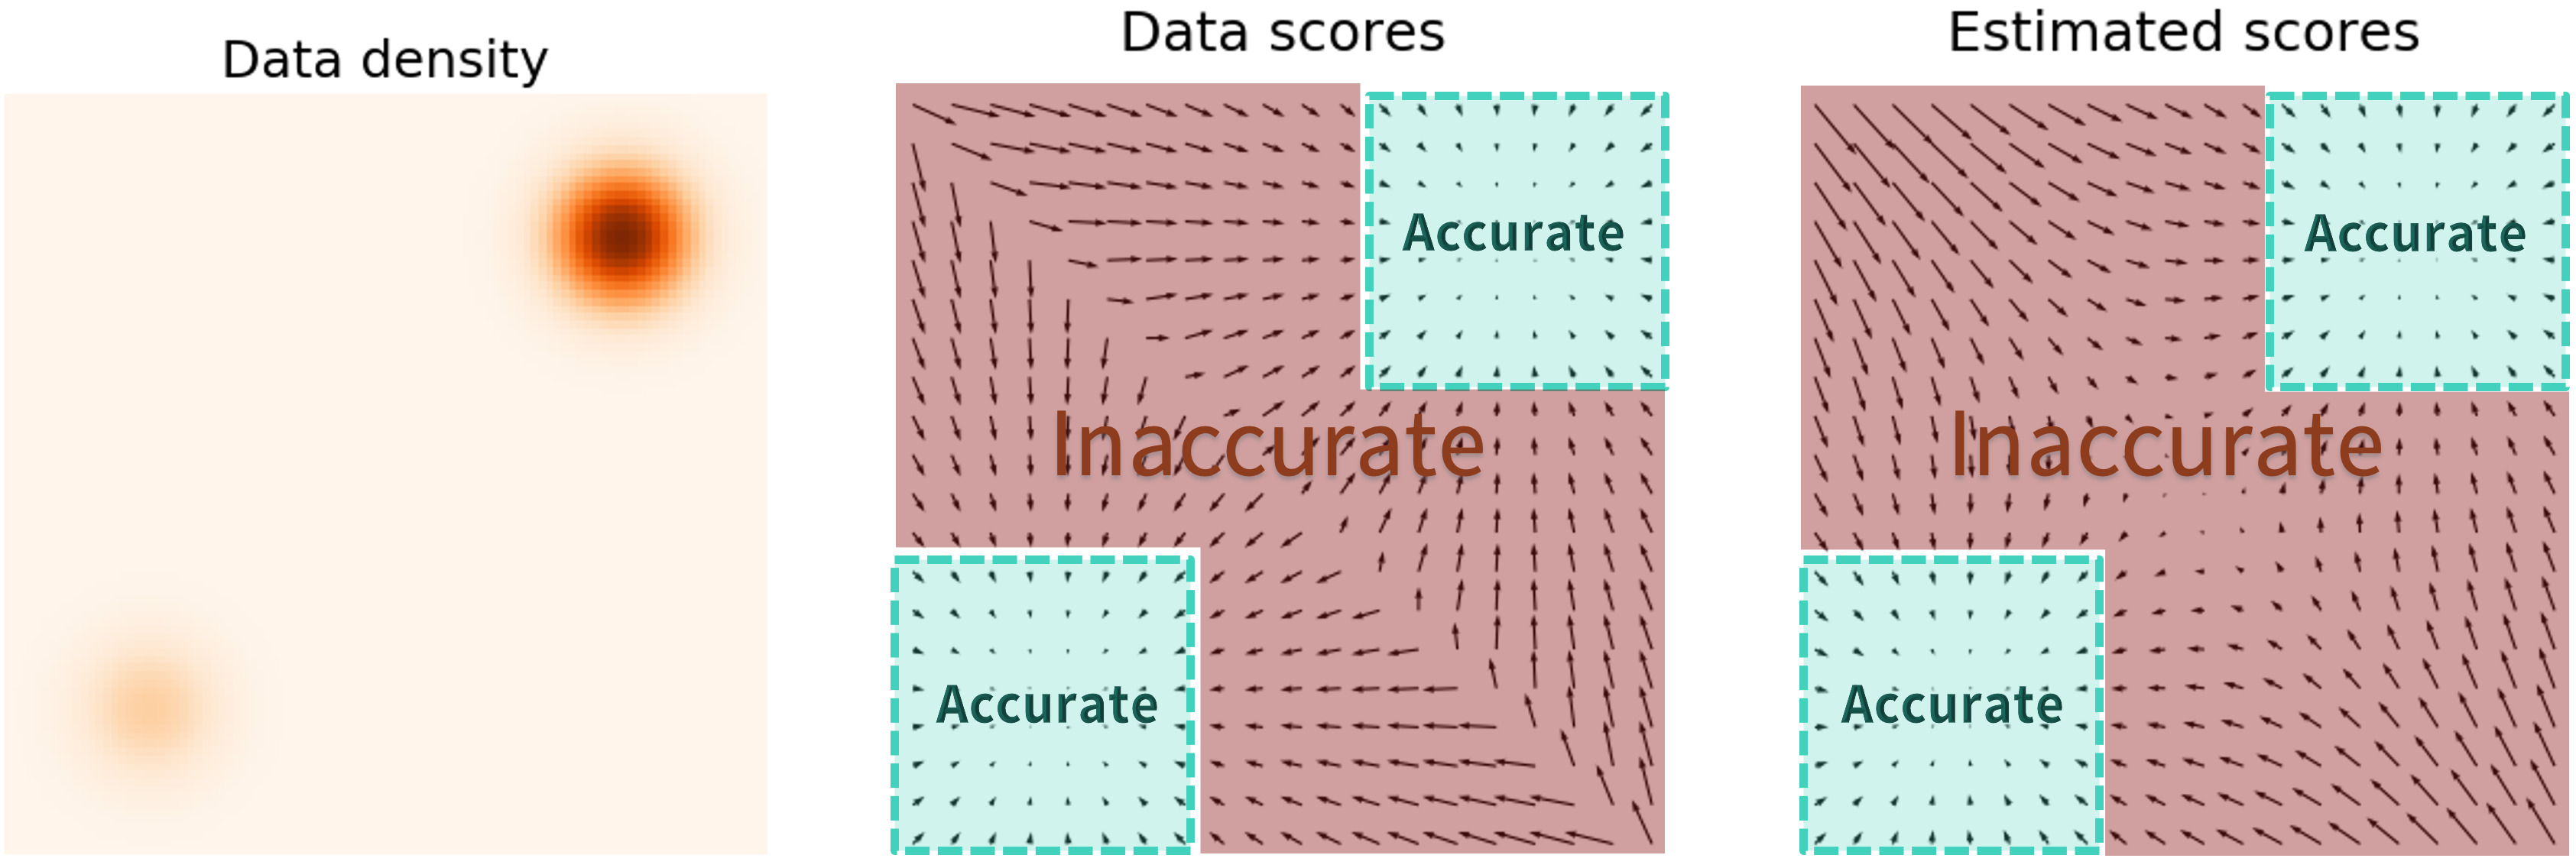
\includegraphics[width=0.8\linewidth]{gfx/low_density_probs.png}
    \caption{Score estimation for low density regions in the case of Gaussian mixtures. Source : \url{https://yang-song.net/blog/2021/score/}}
    \label{fig:low_d_estimation}
\end{figure}
This raises the following question : \textbf{How can one account for accurate estimation of the score in low density regions ?}
\subsection{Injecting more noise}
In order to account for accurately estimating the score for regions with low density, \citep{song2020generativemodelingestimatinggradients} propose to inject noise in several scales to the data points. When the noise scale $\sigma$ is sufficiently high, regions with low density for distribution $P$ are more likely to be populated for distribution $P_{\Sigma}$. This induces a trade-off between the magnitude of the added noise, i.e the size of $\sigma$, which populates the low density regions, and the alteration to the data distribution. In order to circumvent this issue, \citep{song2020generativemodelingestimatinggradients} propose \textit{annealed Langevin dynamics}, which consists in altering data with several noise scales $\sigma_{1},\sigma_{2},\ldots \sigma_{L}$, and training the model to minimize the following sum of score matching losses at different noise scales : 
\begin{equation}\label{eq:annealed_langevin}
    J_{ASM}(\theta) = \sum_{i=1}^{L} \lambda(i)E_{p_{\sigma_{i}}}\left[ ||\nabla \log p(x) - s_{\theta}(x,i)||^{2}  \right]
\end{equation}
where $\lambda(i)$ is a weighting schedule, and $s_{\theta}(x,i)$ is a model that takes in input the current point and the scale of the added noise. Note that the terms in equation \ref{eq:annealed_langevin} can be approximated using the aforementioned score matching techniques.
Once a model is trained to minimize $J_{ASM}$, the sampling procedure generating samples from $\hat{P}$ is described by algorithm \ref{algo:ald}.
\begin{algorithm}
\caption{Annealed Langevin Dynamics for Sampling \citep{song2020generativemodelingestimatinggradients}}
\begin{algorithmic}[1]\label{algo:ald}
\Require{Sequence of noise levels $\{\sigma_i\}_{i=1}^L$, step size $\epsilon$, number of iterations $T$}
\State Initialize $x_0$
\For{$i \leftarrow 1$ to $L$}
    \State Set step size $\alpha_i \leftarrow \epsilon \cdot \frac{\sigma_i^2}{\sigma_L^2}$
    \For{$t \leftarrow 1$ to $T$}
        \State Draw $z_t \sim \mathcal{N}(0, I)$
        \State Update $x_t \leftarrow x_{t-1} + \frac{\alpha_i}{2} s_\theta(x_{t-1}, \sigma_i) + \sqrt{\alpha_i} z_t$
    \EndFor
    \State Set $x_0 \leftarrow x_T$
\EndFor
\State \textbf{return} $x_T$
\end{algorithmic}
\end{algorithm}
\citep{sohldickstein2015deepunsupervisedlearningusing,ho2020denoisingdiffusionprobabilisticmodels} proposed a similar framework that was labeled as \textit{denoising diffusion probabilistic models}. Akin to \citep{song2020generativemodelingestimatinggradients}, they propose a noise scale $\beta{1},\beta{2},\ldots,\beta_{L}$, and they create a Markov chain for each training point $x_{0} \rightarrow \{x_{0},x_{1},\ldots,x_{L}\}$, where each $x_{i} \sim \mathcal{N}(\sqrt{1-\beta_{i}}x_{i-1},\beta_{i}I_{d})$, thus $x_{i} \sim \mathcal{N}(\sqrt{\alpha_{i}}x_{0},(1-\alpha_{i})I_{d})$, with $\alpha_{i} = \prod_{k=1}^{i}(1-\beta_{k})$. By denoting $p(x_{i}|x_{0}) = \mathcal{N}(x_{i}|\sqrt{\alpha_{i}}x_{0},(1-\alpha_{i})I_{d})$, a noise conditional model $s_{\theta}(\Tilde{x},i)$ is trained to minimize the following objective, that is similar to the one described by equation \ref{eq:annealed_langevin} : 
\begin{equation}\label{eq:ddpm}
    \mathcal{J}_{DDPM}(\theta) = \sum_{i=1}^{L} (1-\alpha_{i})\mathbb{E}_{p} \left[ \mathbb{E}_{p(.|x)}\left[ ||s_{\theta}(\Tilde{x},i) - \nabla \log p(x_{i}|x)||^{2} \right]  \right]
\end{equation}
The sampling process is done by starting from $x_{L} \sim \mathcal{N}(0,I_{d})$, then reversing the Markov chain :
\begin{equation}
    x_{i-1} = \frac{1}{1-\beta_i} \left( x_i + \beta_i s_\theta(x_i, i) \right) + \sqrt{\beta_i} z_i
\end{equation}
with $z_{i} \sim \mathcal{N}(0,I_{d})$ and $i \in \{L,\ldots,1\}$.
The generative procedure described by \citep{ho2020denoisingdiffusionprobabilisticmodels} is an alternative to using Langevin dynamics for generating samples using an estimated score, but one sees numerous similarities with the method proposed by \citep{song2020generativemodelingestimatinggradients}. Notably, both methods use increasing noise schedules to perturb the points, and estimate a noise conditional score model. One can thus ask : \textbf{Is there a unifying framework for generating with noise conditional score models ?}
\subsection{Diffusion process}
The answer to this question was obtained by answering another question : What happens when $L \rightarrow \infty $, i.e when the number of noise scales is infinite ? 
\\
When $L \rightarrow \infty$, the number of perturbations can be viewed as continuous and increasing noise perturbations. Thus, this can be seen as a stochastic process, and can sometimes be the solution of stochastic differential equations (SDEs). In order to generalize the idea of denoising score matching to continuous noise injections, we can mention diffusion processes. 
Diffusion processes are derived from modeling the dynamics of molecular systems, particularly from the theory of Langevin dynamics. In summary, a simplified model of a system can be created by compensating the omitted degrees of freedom through stochastic differential equations.
Fundamentally, a diffusion process $\{x_{t}\}_{t=0}^{T}$ is a Markov process indexed by a continuous time variable $t \in [0,T]$. By adding iteratively  noise to the samples, one can describe the \textit{forward} diffusion process as a solution the following Itô SDE : 
\begin{equation}\label{eq:forward_diff}
    dx = f(x,t)dt + g(t)dw 
\end{equation}
where dw is the standard Wiener process (Brownian motion). $f(x,t)$ is called the \textit{drift} coefficient of $x(t)$ and $g(t)$ is called the \textit{diffusion} coefficient of $x(t)$. The distribution of $x_{T}$  when $T \rightarrow \infty$ is called the \textit{prior} distribution and can be carefully chosen by tailoring $f$ and $g$ in the aforementioned SDE \citep{song2021scorebasedgenerativemodelingstochastic}.
Equation \ref{eq:forward_diff} has a unique solution when the drift and diffusion coefficients are Lipschitz in all of their arguments \citep{oksendal2003stochastic}. Generally, one chooses $f$ and $g$ such that $p_{T}$ is an easy distribution to sample from, like a zero-mean isotropic Gaussian distribution. 
For instance, with a linear drift $f(x) = -x$ and a constant diffusion coefficient $g(t) = \sqrt{2}$, one has that $p_{T}$ converges exponentially fast to $\mathcal{N}(0,I_{d})$ (CITATION).
In the following, we denote $P_{t}$ as the distribution of a sample from $P$ at timestep $t$. We also denote by $p_{t}(x_{t}|x_{0})$ the conditonal distribution of a noisy point $x_{t}$ after starting with point $x_{0}$.
When does the score intervene in this case ? \citep{ANDERSON1982313} proves that the reverse of a diffusion process, starting at distribution $P_{T}$ and ending in distribution $P$ is also a diffusion process, solution to the following SDE, that we label as the \textit{backward SDE} : 
\begin{equation}\label{eq:backward_diffusion}
    dx = \left(f(x,t) - g(t)^{2}\nabla \log p_{t}(x)dt\right) + g(t)dw
\end{equation}
Thus, if one learns $\nabla \log p_{t}(x)$ for $t \in [0,T]$, one can sample from $P$ by first sampling a point from $P_{T}$ and solving equation \ref{eq:backward_diffusion}.
\citep{song2021scorebasedgenerativemodelingstochastic} propose thus a continuous version of the discrete noise conditional score estimation, with the following objective function : 
\begin{equation}
    J_{\text{CSM}}(\theta) =\mathbb{E}_{t} \left[ \lambda(t) \mathbb{E}_{P} \left[ \mathbb{E}_{P_{t}} \frac{1}{2} \left\| s_{\theta}(x_{t},t) - \nabla_\mathbf{x} \log p_{t}(x_{t}|x) \right\|^2 \right]\right]
\end{equation}
Once the score is accurately estimated, one can solve the backward SDE using $s_{\theta}(x,t)$ as an estimator for $\nabla \log p_{t}(x)$. Several solving schemes are available, notably numerical solvers that discretize the backward SDE such as the stochastic Runge-Kutta and Euler-Maruyama methods \citep{kpj1992numerical}. Algorithm \ref{algo:sample_diffusion} describes this sampling procedure using the Euler Maruyama sampler. Furthermore, \citep{song2021scorebasedgenerativemodelingstochastic} proposed a different sampling method by using the corresponding deterministic reverse process, labeled as the \textit{probability flow} ordinary differential equation (ODE). It is expressed as : 
\begin{equation}\label{eq:backwatd_ode}
    dx = f(x,t) - \frac{1}{2}g(t)^{2}\nabla \log p_{t}(x)dt
\end{equation}
and can be equivalently solved by ODE numerical solvers that discretize the ODE. This version provides a computational advantage as less discretization steps are needed for a fair quality, but there is a tradeoff between image quality by SDE generation and the number of function evaluations (computation cost) via ODE generation \citep{xu_restart_2023}. 

\begin{multicols}{2}

\begin{algorithm}[H]
\caption{Training a Score-based Diffusion Model}
\begin{algorithmic}[1]\label{algo:train_diffusion}
\Require{Dataset $\mathcal{D}$, learning rate $\eta$}
\State Initialize parameters $\theta$
\While{not converged}
    \State Sample mini-batch $\{x^{(i)}\}$ from $\mathcal{D}$
    \State Update $\theta \gets \theta - \eta \nabla_\theta \mathcal{J}_{CSM}(\theta)$
\EndWhile
\State \Return{Trained model parameters $\theta$}
\end{algorithmic}
\end{algorithm}

\columnbreak

\begin{algorithm}[H]
\caption{Sampling via Discretized Backward SDE}
\begin{algorithmic}[1]\label{algo:sample_diffusion}
\Require{Trained parameters $\theta$, number of steps $N$, time horizon $T$}
\State Initialize $x_T \sim p_T(x)$ (e.g., Gaussian)
\State Initialize current timestep $t_{n} = T$
\For{$n = N$ down to $1$}
    \State Set time step $\Delta t = T / N$
    \State Update current timestep $t_{n} = t_{n} - \Delta t$
    \State Sample noise $\epsilon_n \sim \mathcal{N}(0, I)$
    \State Update using backward SDE discretization:
    \[
    x_{n-1} = x_n - s_\theta(x_n, t_n) \Delta t + \sqrt{\Delta t} \epsilon_n
    \]
\EndFor
\State \Return{Sample $x_0$}
\end{algorithmic}
\end{algorithm}

\end{multicols}
\citep{karras2022elucidatingdesignspacediffusionbased} proposed a unifying framework for diffusion-based generative models, and showed that different sampling schemes can be used with the same diffusion model. 
Table \ref{tab:diffusion_table} lists a few configurations for popular diffusion based generative models. 

\begin{table}[ht]
\centering
\caption{Specific design choices employed by different model families}
\begin{tabular}{@{}m{1.5cm}m{4cm}m{4cm}m{4cm}@{}}\label{tab:diffusion_table}
\toprule
\textbf{Model} & \textbf{VP} \citep{song2020generativemodelingestimatinggradients} & \textbf{VE} \citep{ho2020denoisingdiffusionprobabilisticmodels} & \textbf{EDM \citep{karras2022elucidatingdesignspacediffusionbased}} \\
\midrule
\textbf{ODE Sampling} & Euler & Euler & 2nd order Heun \\
\textbf{Time steps $t_i$} & $1+\frac{i(1-\epsilon_{0})}{N-1}$ & $\sigma^{2}_{max}\left(\frac{\sigma_{min}^2}{\sigma_{max}^2}\right)^{\frac{i}{N-1}}$ & $t$ \\
\midrule
\textbf{Training (Sec. 5)} & & & \\
\textbf{Noise distribution} & $\sigma^{-1}(\sigma) \sim \mathcal{U}(\epsilon_{t},1)$ & $\ln(\sigma) \sim \mathcal{U}(\ln(\sigma_{min}), \ln(\sigma_{max}))$ & $\ln(\sigma) \sim \mathcal{N}(P_{mean}, P_{std}^2)$ \\
\textbf{Loss weighting $\lambda(\sigma)$} & $\frac{1}{\sigma^2}$ & $\frac{1}{\sigma^2}$ & $\left(\frac{\sigma^2 + \sigma^2_{data}}{\sigma \cdot \sigma_{data}}\right)^2$ \\
\bottomrule
\end{tabular}
\end{table}
Thus, diffusion appears as a viable choice for approximating probability distributions. However, as most distribution approximation methods, estimation errors arise in practice. For the diffusion framework, there is two main sources of error : \textbf{approximation} errors related to the training of the score, and \textbf{sampling} errors related to the discretization of the backward ODE or SDE. \citep{lai2023fpdiffusionimprovingscorebaseddiffusion,chao2023investigatingconservativepropertyscorebased} notably showed that diffusion models in practice are not conservative for large values of $t$, i.e does not define vector fields of real valued functions.
This poses a new challenge, which is to mitigate the error sources related to estimation. As generation consists of both training and sampling, this calls for improvement during both the training and the sampling stages. Thus, we ask the following question : \textbf{How to refine the generative process ?} In the following section, we will answer this broadly for generative models and specifically provide an answer for diffusion models in sections \ref{sec:dg} and \ref{sec:rl}.
By noting $\Tilde{P}$ the distribution induced by training a generic generative model and sampling from it, one can check a discrepancy measure between the two distributions (Definition \ref{def:divergence}) to evaluate \textit{how accurate} the estimation procedure is. In our work, we will focus on the family of f-divergences, that compute the following metric with respect to the Lebesgue measure : 
\begin{equation}
    D_{f}(\Tilde{P}||P) = E_{P}\left[f(\frac{P}{Q})\right] = \int p(x)f(\frac{p(x)}{\Tilde{p}(x)}dx
\end{equation}
\section{Expressivity of a generative model}
\label{sec:related:improve_generation}
The sources of error of interest in our case are the expressivity of the considered model, and the stopping iteration. When the number of iterations goes to infinity, the expressiveness of the family of parameters yield an optimal distribution $\Tilde{P}$ for a given f-divergence, that is not necessarily equal to $P$. One controls the expressivity of a model by architecture design, choice of the objective function, and training paradigm. 
\subsection{Precision and recall as f-divergences}\label{subsec:precision_recall}
For generative models in general, the choice of an $f$ in the minimization of an $f$-divergence yields different results in practice, for the same family of models. For instance, \citep{minka2005divergence} observed that optimizing Kullback-Leibler divergence( $f(x) = x \log x$) tends to favor \textit{mass-covering} models and that optimizing the reverse KL ($f(x) = -\log x$) and Jensen-Shannon $f(x) = \frac{1}{2}\left( x\log x - (x+1)\log \left( \frac{x+1}{2} \right) \right)$
tends to favor \textit{mode-seeking} behaviors. Here, a mass covering model will produce diverse samples, covering a substantial part of the support of $P$. Conversely, a mode seeking model will display less diversity in the produced samples, but the generated samples will have a high target density $p$, which make them more \textit{precise}.
Depending on the use case, one would either want to produce samples of high quality or with high diversity. For example, using generative models for drug discovery would require precise samples, while using them to generate images for artistic synthesis might allow less precision for more diversity. INSERT PLOT HERE LIKE FIGURE 4.3 from alex thesis. This implicit trade-off was investigated by \citep{verine2024precision} in the context of GANs and normalizing flows, and they derive a new divergence, termed as the precision and recall (P\&R) divergence, that is dependent on a specified trade-off parameter $\lambda$. It is essentially an $f$-divergence, with a function $f_{\lambda}$ defined as : 
\begin{equation}
  f_{\lambda}(x) =
  \begin{cases} 
    \max(\lambda x,1) - \max(\lambda,1) & \text{if } \lambda \in [0,+\infty[ \\
    \mathbf{1}_{x=0} & \text{if } \lambda = +\infty.
  \end{cases}
\end{equation}
In order to control the expressivity of a generative model with a specified trade-off between diversity and precision, \citep{verine2024precision} propose a method for GANs and normalizing flows, that improves upon the traditional framework of $f$-GANs introduced by \citep{nowozin2016fgantraininggenerativeneural}.
Modifying the objective functions is thus a foundational method to control the expressivity of a generative model. This, in practice however, is not directly applicable to diffusion models as the loss is not expressed as an $f$-divergence, but rather as a score matching loss. In the following subsections, we will give examples that improve the expressivity of a score based model.


\subsection{Using the theory of diffusion as a refinement process}
We will give two examples that improved the likelihood of the generated distribution of diffusion models. One is based on conservativity, a fundamental property that the estimated score should satisfy, and another is based on the FOkker-Planck equation, that is related to the SDE formulation of score based models.
\begin{definition}
    A vector field, represented by a \textit{vector} valued function $v : \mathcal{X} \rightarrow \mathbb{R}^{d}$, is said to be conservative if it can be expressed as the gradient of a real valued function
\end{definition}
By definition, the ground truth score $s(x,t) = \nabla_{x} \log p_{t}(x)$ is thus conservative. However, \citep{salimans2021should,chao2023investigatingconservativepropertyscorebased} highlighted that notable diffusion models, that are defined as U-Nets in practice, are not conservative. In order to ensure conservativity, \citep{salimans2021should,saremi2018deepenergyestimatornetworks} propose to constrain the architecrure of the model such that its output vector field is modeled as a gradient of a real valued function. This, however, constrains the expressivity of the architecture overall. \citep{chao2023investigatingconservativepropertyscorebased}, on the other hand, add a regularization term based on higher orders of the score to ensure the conservativity. This method allowed for more flexible architecture choices, and an improvement in likelihood computations of the estimated distributions. We will now present another method that helped enforce conservativity, introduced by \citep{lai_fp-diffusion_2023}.
The ground truth density $p_{t}$ associated to the forward diffusion SDE (equation \ref{eq:forward_diff}) satisfies the Fokker-Planck equation \citep{oksendal2003stochastic} : 
\begin{equation}\label{eq:fokker_plack}
  \frac{\partial p_t(x)}{\partial t} = -\frac{\partial}{\partial x} \left[ f(x, t) p_t(x) \right] + \frac{\partial^2}{\partial x^2} \left[g(t) p_t(x) \right]
\end{equation}
\citep{lai_fp-diffusion_2023} derive from this equation another equation that the ground truth score should satisfy, labeled as \textbf{the score FPE} (c.f Proposition 3.1 and Appendix G in \citep{lai_fp-diffusion_2023}) : 
\begin{equation}\label{eq:score_fpe}
    \frac{\partial s(x,t)}{\partial t} = \nabla_{x}\left[\frac{1}{2}g^{2}(t)\mathrm{div}_{x}(s(x,t)) + \frac{1}{2}g^{2}(t)\left|\left|s(x,t)\right|\right|^{2} - \langle f(x,t),s(x,t) \rangle - \mathrm{div}_{x}(f(x,t))\right]
\end{equation}
where $s(x,t) = \nabla_{x} \log p_{t}(x)$ denotes the ground truth score, and $\mathrm{div}_{x}(s(x,t))= \sum_{i=1}^{d}\frac{\partial s(x,t)}{\partial x_{i}} $ denotes the divergence of the vector field $s(x,t)$. In practice, it is observed that most trained diffusion models do not satisfy the score FPE. By denoting by $\mathcal{R}(.) $ as the linear mapping corresponding to the right hand side of equation \ref{eq:score_fpe}, one can define a \textit{residual} $\epsilon_{\theta}$ corresponding to the difference $\frac{\partial s_{\theta}(x_{t},t)}{\partial t} - \mathcal{R}[s_{\theta}](x_{t},t) $, evaluating how far the current estimated score is from satisfying the score FPE. This residual is added as a regularization term in various forms, depending on the used score matching loss, and thus enforces the score FPE to be satisfied.
\citep{lai_fp-diffusion_2023} demonstrate that notable implications of satisfying equation \ref{eq:score_fpe} are : 
\begin{itemize}
    \item Reducing the KL divergence between the target distribution $P_{0}$ and the estimated density with ODE sampling (solved by discretization of equation \ref{eq:backwatd_ode})
    \item Enforcing the conservativity of the vector field $s_{\theta}(x_{t},t)$
\end{itemize}
These methods elaborate a novel framework that is suitable for a more theoretically grounded training for diffusion based models. One of the immediate setbacks of adopting these methods is their incompatibility with pre trained models, that already display a good performance. We thus ask : \textbf{Are there methods that improve the generative process without retraining a model from scratch ? cCan they be used for a wide array of models ?}
\subsection{Fine-tuning methods}
\citep{lucic2019highfidelityimagegenerationfewer} first noticed that when a GAN is generating data in a label limited setting, there was a significant advantage in using class labels during generation. Using this idea, \citep{dhariwal2021diffusionmodelsbeatgans} presents a boosting method for diffusion models, by incorporating class-specific information during the sampling process through a classifier. This idea was presented in order to make diffusion models increase their precision at the expense of their diversity (c.f subsection \ref{subsec:precision_recall}.
Specifically, given a specified class $y$, one can train a classifier with a parameterized model $c_{\phi}$ to estimate $\nabla \log p(y|x_{t},t)$ for every perturbed point $x_{t}$ at every diffusion step $t$. Then, the sampling transition is done by replacing $p(x_{t}|x_{t+1})$ by $p(x_{t}|y,x_{t+1})$, i.e the score approximation becomes $s_{\theta}(x_{t},t) + \lambda c_{\phi}(x_{t},t,y)$, where $\lambda$ is a scaling parameter that determines the influence of classifier guidance. This technique is not involved in the training of the diffusion model, and can be used as a \textit{refinement} method for fine-tuning the diffusion model. Notably, it can present advantages in terms of computational resources, as a smaller model can be used as a classifier. We will be exploring another boosting method, namely discriminator guidance, as a main improvement framework for diffusion models in chapter \ref{sec:dg}.


\fbox{\parbox{\linewidth}{\textbf{Note :} This method was further extended by \citep{ho2022classifierfreediffusionguidance} to \textit{classifier-free} guidance, by simultaneously training a model on samples x and a context $c$. This is a boosting-free method as only the training procedure is affected, and no additional model is trained. Stable diffusion \citep{rombach2022highresolutionimagesynthesislatent}, among others, used this method during its training, which explains its ability to generate data from user defined prompts.
Adding context information is thus a viable technique to improve the generative process. }}
\\
Another family of methods consists in using statistical sampling algorithms to improve the likelihood of a sample. In the following, we will describe rejection algorithms for generative models, as they rely on density ratio estimation techniques that will be important for the following chapters, notably chapters \ref{sec:dg} and \ref{sec:rl}. 
Rejection sampling \citep{vonN51} is a method for sampling from a target distribution $P$ using a proposal distribution $Q$ and a density ratio $\frac{p(x)}{q(x)}$ between both distributions. In the context of generative models, the idea is to create a new distribution $\Hat{P}$ from the estimated distribution $\Tilde{P}$ by using accepting or rejecting samples from $\Tilde{P}$ with a rejection probability $a(x)$. The resulting density is given by $\hat{p}_{a}(x) = \frac{\Tilde{p}(x)a(x)}{Z}$, where $Z$ is a normalization constant. Thus, the rejection rate is given by $\mathbb{E}_{\Tilde{P}}[a(x)] = \frac{1}{Z}$ or in other terms, one needs to draw $\frac{1}{Z}$ samples in average from $\Tilde{P}$ to have one sample accepted.
\begin{algorithm}
\caption{Generic Rejection Sampling Algorithm}
\begin{algorithmic}[1] % The number tells where the line numbering should start
\State Generate $x \sim \Tilde{P}$
\State Generate $u \sim \mathcal{U}(0,1)$
\While{$u \leq a(x)$} \Comment{Rejection criterium}
    \State $x \sim \Tilde{P}$
    \State $u \sim \mathcal{U}(0, 1)$ \Comment{Draw a uniform random number}
\EndWhile
\end{algorithmic}
\end{algorithm}
In order to exactly match the target density $p(x)$, the literature has proposed an optimal rejection rate $a(x)$ of the form : 
\begin{equation}\label{eq:optimal_rejection}
    a_{\mathrm{opt}}(x) = \frac{p(x)}{M\Tilde{p(x)}}
\end{equation}
where $M = \sup_{\mathcal{X}} \frac{p(x)}{\Tilde{p(x)}}$ and the resulting density function of $\Hat{P}_{a_{\mathrm{opt}}}$ is equal to $p$. However, in a high dimensional $\mathcal{X}$, \citep{mackay2003information} showed that $M$ can be very high and thus set a high rejection rate. For example, in the context of BigGAN \citep{brock2019largescalegantraining} trained on the CelebA dataset \citep{liu2015faceattributes} (178×218 images), the rejection rate is as big as $10^{6}$. Thus, a line of work investigates alternative rejection probabilities $a(x)$ to perform rejection sampling in high dimensions.
\\
In the context of GANs, \citep{azadi2019discriminatorrejectionsampling} propose to involve the discriminator in the \textit{generation} process by using it to estimate the density ratio involved in equation \ref{eq:optimal_rejection}. A discriminator model $d$ parameterized by a set of parameters $\phi$ within the framework of $f$-GANs (\citep{nowozin2016fgantraininggenerativeneural},\ref{eq:f_gan}) can be used to estimate the density ratio using the following expression \citep{verine2024precision}: 
\begin{equation}\label{eq:discriminator_density_ratio}
    \frac{p(x)}{\Hat{p}(x)} \approx \nabla f^{*}(d_{\phi}(x)) = r(x)
\end{equation}
where $f^{*}$ denotes the \textit{Fenchel conjugate} of function $f$. In order to lower the rejection rate, \citep{azadi2019discriminatorrejectionsampling} propose to use the following acceptance probability function : 
\begin{equation}\label{eq:acceptance_bounded}
    a_{\gamma}(x) = \frac{r(x)}{r(x)(1-e^{\gamma}) + e^{\gamma}M}
\end{equation}
Negative values of $\gamma$ are used to lower the rejection rate, but no theoretical contributions are given for the choice of $\gamma$. 
Another line of work explores rejection sampling methods under a \textit{budget}. That is, under budget $K$, solve the following optimization problem : 
\begin{align*}\label{eq:budget_rejection_prob}
\min_a \quad & D_f(P \parallel \tilde{P}_a) \\
\text{s.t.} \quad & 
\begin{cases} 
\mathbb{E}_{\hat{P}}[a(x)] \geq \frac{1}{K}, \\
\forall x \in X, \quad 0 \leq a(x) \leq 1.
\end{cases}
\end{align*}
\citep{verine2024optimalbudgetedrejectionsampling} derives an optimal solution for this problem, with a rejection probability of the form : 
\begin{equation}
    a_{\mathrm{K-opt}}(x) = \min \left(\frac{p(x)c_{K}}{\tilde{p(x)}M},1\right)
\end{equation}
where $c_K$ is a constant such that $\mathbb{E}_{\Tilde{P}}[a_{\mathrm{K-opt}}(x)] = \frac{1}{K}$
The density ratio ratio is computed by a discriminator as in \citep{azadi2019discriminatorrejectionsampling}, and the constant $c_{K}$ is computed using dichotomy.

\section{Conclusion}
Diffusion models emerge as a viable family of generative models, as they emanate from a nice theoretical framework. The generation process is two-folds : training a model $s_{\theta}$ to estimate the target score function at each noise level $t in [0,T]$, then use the estimated score to solve the backward SDE (Equation \ref{eq:backward_diffusion}) or ODE (Equation \ref{eq:backwatd_ode}). While this separation allows for separately improving each step of the process, it might represent a concatenation of two error sources : an approximation error related to the training process, and an estimation error related to the sampling process.
Several diffusion models are currently state of the art in generation, and the main question of our work is how to improve these pre-trained models, without retraining them and without additional data. In subsection \ref{sec:diffusion}

This raises the following questions, that we will try to answer in chapter \ref{sec:related:improve_generation}, we presented a few ideas to improve generative models, and booting methods emerged as a viable technique to do so. This raises the following question : 
\begin{itemize}
    \item \textbf{Can classifier guidance be generalized to a boosting method that does not rely on class information ?} This question is answered in chapter \ref{sec:dg}, where we introduce discriminator guidance \citep{kim2023refininggenerativeprocessdiscriminator} and improve the theoretical framework of this method.
    \item \textbf{Can we extract further information from the density ratio estimated by a discriminator ?} This question will be answered in chapter \ref{sec:rl}, where we introduce reinforcement learning methods that uses information from an estimated density ratio as a reward function. 
\end{itemize}
\label{sec:related:conclusion}


